\documentclass{article}
\usepackage{graphicx} % Required for inserting images
\usepackage{authblk} % Required for author affiliations
\usepackage{indentfirst} % Indent first paragraph of sections
\usepackage{amssymb} % For mathematical symbols
\usepackage{amsthm} % For theorem environments
\usepackage{amsmath} % For advanced math typesetting
\usepackage{hyperref}
\usepackage{enumitem}
\usepackage{pgfplots} % For plots
\usepackage{tikz} % For drawing shapes
\usepackage{circuitikz}
\usepackage{float} % For [H] float option
\usepackage{braket}
\usepackage{dsfont}
\pgfplotsset{compat=1.18} % Set compatibility level
\newtheorem{theorem}{Theorem}
\newtheorem{law}{Law}
\newtheorem{principle}{Principle}
\newtheorem{corollary}{Corollary}[theorem]
\newtheorem{lemma}[theorem]{Lemma}
\newtheorem{definition}{Definition}
\newtheorem{problem}{Problem}
\newtheorem{solution}{Solution}
\newtheorem*{example}{Example}
\newtheorem{remark}{Remark}
\newtheorem{proposition}{Proposition}
\newtheorem{result}{Result}
\newcommand{\id}{\mathds{1}}
\reversemarginpar
\hypersetup{
    colorlinks=true,
}
\begin{document}
\title{PHYS 357: Honours Quantum Physics 1}
\author{W.R.YCH.}
\date{August \(31^{st}\), 2026}
\setcounter{Maxaffil}{0}
\renewcommand\Affilfont{\itshape\small}
\maketitle
\noindent\rule{\textwidth}{0.4pt}
\thispagestyle{empty}
\begin{abstract}
\end{abstract}
\noindent\rule{\textwidth}{0.4pt}
\clearpage
\thispagestyle{empty}
{
  \hypersetup{linkcolor=black}
  \tableofcontents
}
\clearpage
\setcounter{page}{1}


\section{Introduction}
Textbook used is JS Townsend, \emph{A Modern Approach to Quantum Mechanics}, 2nd ed., University Science Books 2012. Taught by Bill Coish. Mondays, Wednesdays and Fridays from 9:35 to 10:25 in Steward Biology Building N2/2. Course grading is divided as follows:
\begin{itemize}
    \item 10\% problem sets (must be handwritten scans).
    \item 40\% quizzes (on Wednesdays, best 8 of 12).
    \item 20\% midterms (best of 2, October 2nd and November 6th).
    \item 30\% final exam.
\end{itemize}


\section{Mathematical Background}

\subsection{Taylor expansion}
\begin{definition}[Taylor series]
    A function $f$ that is smooth near $a$ equals the power series
    \begin{equation}
        f(x) = \sum_{n=0}^{\infty}\frac{f^{(n)}(a)}{n!}(x-a)^n,
    \end{equation}
    where $f^{(n)}$ is the $n$th derivative. Expanding about $a = 0$ gives the Maclaurin series.
\end{definition}
\begin{result}[Series used in this course]
    \begin{equation}
        e^{x} = \sum_{n=0}^{\infty}\frac{x^n}{n!}, \qquad
        \cos x = \sum_{n=0}^{\infty}\frac{(-1)^n x^{2n}}{(2n)!}, \qquad
        \sin x = \sum_{n=0}^{\infty}\frac{(-1)^n x^{2n+1}}{(2n+1)!},
    \end{equation}
    together with the binomial theorem $(1+u)^N = \sum_{n=0}^{N}\binom{N}{n}u^n$ for integer $N$.
\end{result}
\begin{remark}
    Comparing the three series gives Euler's formula $e^{i\theta} = \cos\theta + i\sin\theta$, hence
    \begin{equation}
        \cos\theta = \frac{e^{i\theta}+e^{-i\theta}}{2}, \qquad \sin\theta = \frac{e^{i\theta}-e^{-i\theta}}{2i}.
    \end{equation}
    These two are used constantly when rotation matrices are written out.
\end{remark}
\begin{problem}[The exponential as a limit]
    Show that $\lim_{N\to\infty}\left(1+x/N\right)^N = e^x$.
\end{problem}
\begin{remark}
    This limit is what lets a rotation be written as an exponential. A finite rotation is $N$ infinitesimal ones stacked up,
    \begin{equation}
        R(\theta\hat{n}) = \lim_{N\to\infty}\left(\id - \frac{i}{\hbar}\frac{\theta}{N}\,\hat{n}\cdot\vec{S}\right)^{N} = e^{-i\theta\,\hat{n}\cdot\vec{S}/\hbar}.
    \end{equation}
\end{remark}


\section{Stern-Gerlach Experiments}
\marginpar{August 31 - September 9, 2026}

\subsection{The classical picture}

\subsubsection{Angular momentum}
\begin{definition}[Orbital angular momentum]
    The orbital angular momentum of a particle is
    \begin{equation}
        \vec{L} = \vec{r} \times \vec{p},
    \end{equation}
    where $\vec{r}$ is the position vector and $\vec{p} = m\vec{v}$ is the linear momentum.
\end{definition}
For motion confined to the $x$-$y$ plane, only the $z$ component survives. On a circular path of radius $r$ with speed $v$,
\[L_{z} = mvr.\]
\begin{definition}[Angular momentum of a rigid body]
    For a rigid body\footnote{A rigid body is one that does not deform under the action of external forces.} rotating about a fixed axis this is
    \[L = I_{0}\omega,\]
    with $I_{0}$ the moment of inertia and $\omega$ the angular velocity.
\end{definition}
\begin{remark}
    The moment of inertia $I_0$ measures how mass is distributed relative to the rotation axis.
\end{remark}

\subsubsection{Magnetic moment of a circulating charge}
\begin{definition}[Magnetic moment]
    A magnetic moment is a measure of the net circulation of electric charge. It is a vector quantity that determines the torque a magnet will experience in an external magnetic field.
\end{definition}
The magnetic moment of a point particle of mass $m$ and charge $q$ in a circular orbit of radius $r$ and period $T$ is
\[\mu = \frac{IA}{c}\footnotemark = \frac{1}{c}\left(\frac{qv}{2\pi r}\right)\left(\pi r^{2}\right) = \frac{q}{2mc}\,mvr = \frac{q}{2mc}\,L_{z},\]
where $I$ is the current and $A$ is the area enclosed by the orbit. A single circulating charge counts as a steady current $I = q/T = qv/2\pi r$ because it passes any given point on the loop once per period.
\footnotetext{Here $c$ is in Gaussian units.}

\subsubsection{Gyromagnetic ratio}
\begin{definition}[Gyromagnetic ratio]
    The gyromagnetic ratio $\gamma$ is the constant of proportionality between the magnetic moment and the angular momentum,
    \begin{equation}
        \vec{\mu} = \gamma \vec{L}.
    \end{equation}
    For the circulating charge above,
    \begin{equation}
        \gamma = \frac{q}{2mc}.
    \end{equation}
\end{definition}
\begin{remark}
    This is a purely classical result, since the charge is treated as a point particle on a definite orbit with a definite radius and speed, and nothing is quantized. It matters here because measuring $\vec{\mu}$ is how we measure $\vec{L}$, and it is what the Stern-Gerlach apparatus exploits.
\end{remark}

\subsection{Spin}
\begin{definition}[Spin]
    Spin $\vec{S}$ is an intrinsic angular momentum carried by a particle. It is a fixed property of the particle type, like charge or mass, and does not come from any motion through space. A stationary electron alone in empty space still has spin.
\end{definition}
In quantum mechanics the spin $\vec{S}$ replaces the orbital angular momentum $\vec{L}$ of the classical picture.

\subsubsection{Intrinsic moment and the g-factor}
The magnetic moment is still proportional to the angular momentum, but the gyromagnetic ratio picks up an extra dimensionless factor,
\begin{equation}
    \vec{\mu} = \gamma\vec{S}, \qquad \gamma = \frac{qg}{2mc},
\end{equation}
where $g$ is the g-factor of the particle.
\begin{definition}[g-factor]
    The g-factor of a particle\footnote{Its value must be measured or derived from relativistic quantum theory.} is the dimensionless number relating its magnetic moment to its spin angular momentum. It measures how much stronger or weaker the moment is than the classical value $\gamma = q/2mc$, which corresponds to $g = 1$.
\end{definition}

\subsubsection{Magnetons}
\begin{definition}[Planck constant]
    The Planck constant $h$ is the fundamental constant of quantum mechanics. It sets the scale at which quantization matters, and relates the energy of a photon to its frequency by $E = h\nu$. Its value is
    \[h \approx 6.626 \times 10^{-34}\ \mathrm{J\,s}.\]
    It has units of $J\cdot s$, which is the same as angular momentum.
\end{definition}
\begin{definition}[Reduced Planck constant]
    \begin{equation}
        \hbar = \frac{h}{2\pi}.
    \end{equation}
    It carries units of angular momentum, so $[\hbar] = [L_z] = \frac{kg\cdot m^2}{s}$. Its value is $\hbar = 1.055 \times 10^{-27}\ \mathrm{erg\,s} = 6.582 \times 10^{-16}\ \mathrm{eV\,s}$.
\end{definition}
Writing $\vec{S} = \hbar(\vec{S}/\hbar)$ with $\vec{S}/\hbar$ dimensionless, the $\hbar$ joins the gyromagnetic ratio. The combination $q\hbar/2mc$ then carries the units and sets the natural size of the moment at a given mass scale.
\begin{definition}[Bohr magneton]
    The Bohr magneton is the natural unit of magnetic moment for an electron,
    \begin{equation}
        \mu_{B} = \frac{|e|\hbar}{2m_{e}c}.
    \end{equation}
\end{definition}
\begin{definition}[Nuclear magneton]
    The nuclear magneton is the same combination with the proton mass, and is the natural unit for nucleons,
    \begin{equation}
        \mu_{N} = \frac{|e|\hbar}{2m_{p}c}.
    \end{equation}
    Since $m_{p}/m_{e} \approx 1836$, we have $\mu_{N} \approx \mu_{B}/1836$.
\end{definition}
\begin{definition}[Nucleons]
    The subatomic particles that make up the nucleus of an atom, specifically protons and neutrons.
\end{definition}
The electron moment is then written as
\begin{equation}
    \vec{\mu}_{e} = g_{e}\,\mu_{B}\,\frac{\vec{S}}{\hbar},
\end{equation}
and similarly for the proton and neutron with $\mu_{N}$ in place of $\mu_{B}$.

\subsubsection{Values for the electron, proton and neutron}
\begin{table}[H]
\centering
\begin{tabular}{lcccc}
\hline
Particle & Charge $q$ & Mass $m$ & $g$-factor & Gyromagnetic ratio $\gamma$ \\
\hline
Electron & $-|e|$ & $m_{e}$ & $g_{e} \approx 2$ & $g_{e}\mu_{B}/\hbar$ \\
Proton   & $+|e|$ & $m_{p}$ & $g_{p} \approx 5.59$ & $g_{p}\mu_{N}/\hbar$ \\
Neutron  & $0$    & $m_{p}$ & $g_{n} \approx -3.83$ & $g_{n}\mu_{N}/\hbar$ \\
\hline
\end{tabular}
\caption{Charges, masses, g-factors and gyromagnetic ratios.}
\end{table}
\begin{remark}
    The classical derivation gives $\mu = (q/2mc)L_z$, which vanishes when $q = 0$. The neutron is neutral yet has a nonzero moment, so its $\vec{\mu}$ cannot come from a single circulating point charge. This is a first sign that the classical picture fails.
\end{remark}
\begin{remark}
    Since $m_{p} \gg m_{e}$, we get $\mu_{N} \ll \mu_{B}$ and therefore $|\vec{\mu}_{p}| \ll |\vec{\mu}_{e}|$. Stern-Gerlach deflection of nuclei is much weaker than for electrons.
\end{remark}

\subsection{The Stern-Gerlach apparatus}
\begin{definition}[Stern-Gerlach apparatus]
    A device that measures one component of a particle's magnetic moment. A beam of neutral atoms passes through a magnet shaped to produce a strong field gradient along a chosen axis, here $z$. The gradient deflects each atom by an amount proportional to $\mu_z$, and a screen records where it lands. Since $\vec{\mu} = \gamma\vec{S}$, the position on the screen is a direct measurement of $S_z$.
\end{definition}
\begin{figure}[H]
    \centering
    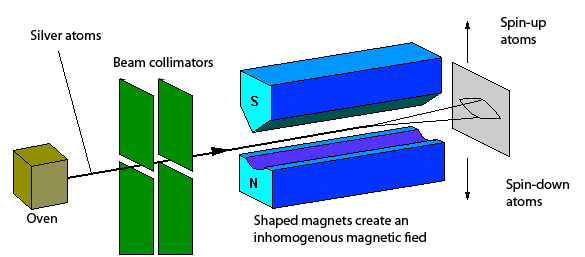
\includegraphics[width=0.5\textwidth]{../Images/Stern-Gerlach_apparatus.png}
    \caption{Illustration of the Stern-Gerlach apparatus.}
    \label{fig:stern-gerlach-apparatus}
\end{figure}

\subsubsection{Force in an inhomogeneous field}
A magnetic moment in a field has potential energy
\begin{equation}
    U = -\vec{\mu}\cdot\vec{B},
\end{equation}
so the force on it is
\[\vec{F} = -\vec{\nabla}U = \vec{\nabla}(\vec{\mu}\cdot\vec{B}), \qquad F_{z} = -\frac{\partial U}{\partial z} = \mu_{z}\frac{\partial B_{z}}{\partial z}.\]
\begin{definition}[Deflection]
    The displacement of an atom on the screen, perpendicular to the beam axis, produced by $F_z$ acting over the length of the magnet. It is proportional to $\mu_z$, so the pattern on the screen is a record of the moments in the beam.
\end{definition}
\begin{remark}
    A uniform field gives no force, only a torque. Thus, the apparatus needs a field \emph{gradient} to deflect anything.
\end{remark}

\subsubsection{Silver atoms}
Silver is used because its net orbital angular momentum vanishes, $\vec{L} = 0$, while $\vec{S} \neq 0$. The entire magnetic moment comes from a single unpaired valence electron, so the atom behaves as one electron spin. For the electron,
\[\mu_{z} = -\frac{g_{e}|e|}{2m_{e}c}\,S_{z},\]
and therefore
\[F_{z} = \mu_{z}\frac{\partial B_{z}}{\partial z} = -g_{e}\frac{|e|}{2m_{e}c}\,S_{z}\,\frac{\partial B_{z}}{\partial z} = g_{e}\frac{|e|}{2m_{e}c}\left|\frac{\partial B_{z}}{\partial z}\right| S_{z},\]
where the last equality assumes $\partial B_{z}/\partial z < 0$.
\begin{result}
    \[F_{z} \propto S_{z}.\]
    The deflection of an atom measures the $z$ component of its spin directly.
\end{result}

\subsubsection{The classical prediction}
Spin is a vector,
\[\vec{S} = (S_{x}, S_{y}, S_{z})^{T}, \qquad S_{z} = |\vec{S}|\cos\theta.\]
\begin{remark}
    The spins leaving the oven point in random directions, so $\theta$ takes every value in $[0,\pi]$ across the beam and $S_z = |\vec{S}|\cos\theta$ takes every value in $[-|\vec{S}|,|\vec{S}|]$. Since $F_z \propto S_z$, each atom is deflected differently and the screen should show a continuous smear, but it shows two spots.
\end{remark}

\subsubsection{The observed result}
\begin{result}[Quantization of spin]
    The electron spin angular momentum is quantized:
    \begin{equation}
        S_{z} = \pm\frac{\hbar}{2}.
    \end{equation}
    The beam splits into two spots.
\end{result}
\begin{definition}[Spin quantum number]
    The spin quantum number $s$ labels the magnitude of a particle's spin and is fixed by the particle type. It takes the values $s = 0, \tfrac12, 1, \tfrac32, \dots$, and a measurement of $S_z$ then gives one of $2s+1$ outcomes,
    \begin{equation}
        S_z = m\hbar, \qquad m = -s, -s+1, \dots, +s.
    \end{equation}
    The electron has $s = \tfrac12$, so $S_z = \pm\hbar/2$ and the beam splits in two. A spin-1 particle would split into three beams, $S_z = +\hbar, 0, -\hbar$.
\end{definition}
\begin{remark}
    Everything in these notes is the $s = \tfrac12$ case, so the state space is two-dimensional. Note also that $S_z$ is a component, while the magnitude is $|\vec{S}| = \hbar\sqrt{s(s+1)}$, which for the electron is $\hbar\sqrt{3}/2$, not $\hbar/2$.
\end{remark}
\begin{definition}[Basis state]
    One of a set of states $\{\ket{j}\}$ that are mutually orthonormal and span the space, so that every state is a unique linear combination of them. For spin-$\tfrac12$ the two outcomes of any one measurement, $\{\ket{\pm\hat{n}}\}$, form a basis.
\end{definition}
\begin{definition}[Ket notation]
    A ket $\ket{\,\cdot\,}$ labels a quantum state as a vector in a vector space. For electron spin the two measurement outcomes give the basis states
    \[\ket{\uparrow} \; \text{for } S_{z} = +\frac{\hbar}{2}, \qquad \ket{\downarrow} \; \text{for } S_{z} = -\frac{\hbar}{2}.\]
    The space is two-dimensional, so any spin state is a linear combination of the two.
\end{definition}
\begin{remark}
    From here on we follow Townsend and write $\ket{+\hat{z}} \equiv \ket{\uparrow}$ and $\ket{-\hat{z}} \equiv \ket{\downarrow}$. The same labels work for any axis: $\ket{\pm\hat{x}}$ are the states with $S_x = \pm\hbar/2$.
\end{remark}

\subsection{Sequential Stern-Gerlach experiments}
\begin{proposition}
    We write SG$z$ for a device whose gradient points along $z$, and SG$x$ for the same device rotated by $90^\circ$ about the beam axis.
\end{proposition}
\begin{definition}[Filter]
    Each device sends atoms into two beams. A filter is a device that blocks one of the beams.
\end{definition}
\begin{remark}
    A beam straight from the oven always splits 50/50 in any SG device, whatever its orientation.
\end{remark}
\begin{figure}[H]
\centering
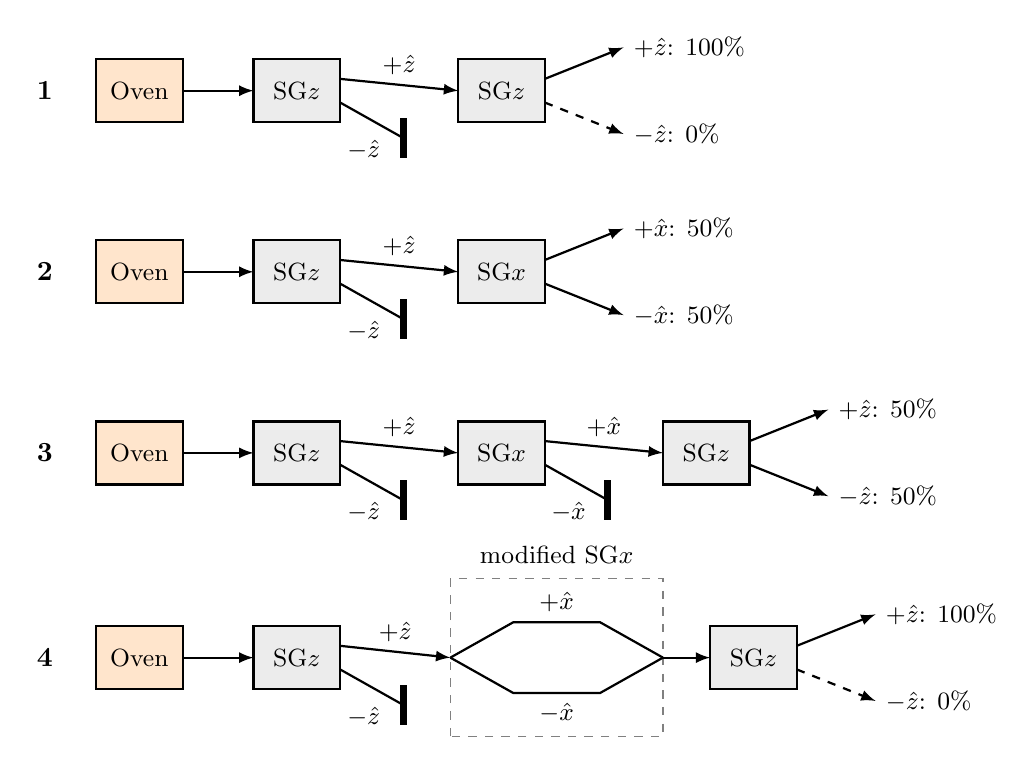
\begin{tikzpicture}[
    box/.style={draw, thick, minimum width=1.1cm, minimum height=0.8cm, font=\small},
    oven/.style={box, fill=orange!20},
    sg/.style={box, fill=gray!15},
    beam/.style={-latex, thick},
    blocked/.style={line width=2.5pt},
    lab/.style={font=\small}
]
% ---------------- Experiment 1 ----------------
\node[font=\bfseries] at (-1.2,0) {1};
\node[oven] at (0,0) {Oven};
\node[sg]   at (2.0,0) {SG$z$};
\node[sg]   at (4.6,0) {SG$z$};
\draw[beam] (0.55,0) -- (1.45,0);
\draw[beam] (2.55,0.15) -- node[lab,above] {$+\hat{z}$} (4.05,0);
\draw[thick] (2.55,-0.15) -- (3.35,-0.6);
\draw[blocked] (3.35,-0.85) -- (3.35,-0.35);
\node[lab] at (2.85,-0.75) {$-\hat{z}$};
\draw[beam] (5.15,0.15) -- (6.15,0.55) node[lab,right] {$+\hat{z}$: 100\%};
\draw[beam, dashed] (5.15,-0.15) -- (6.15,-0.55) node[lab,right] {$-\hat{z}$: 0\%};
% ---------------- Experiment 2 ----------------
\begin{scope}[yshift=-2.3cm]
\node[font=\bfseries] at (-1.2,0) {2};
\node[oven] at (0,0) {Oven};
\node[sg]   at (2.0,0) {SG$z$};
\node[sg]   at (4.6,0) {SG$x$};
\draw[beam] (0.55,0) -- (1.45,0);
\draw[beam] (2.55,0.15) -- node[lab,above] {$+\hat{z}$} (4.05,0);
\draw[thick] (2.55,-0.15) -- (3.35,-0.6);
\draw[blocked] (3.35,-0.85) -- (3.35,-0.35);
\node[lab] at (2.85,-0.75) {$-\hat{z}$};
\draw[beam] (5.15,0.15) -- (6.15,0.55) node[lab,right] {$+\hat{x}$: 50\%};
\draw[beam] (5.15,-0.15) -- (6.15,-0.55) node[lab,right] {$-\hat{x}$: 50\%};
\end{scope}
% ---------------- Experiment 3 ----------------
\begin{scope}[yshift=-4.6cm]
\node[font=\bfseries] at (-1.2,0) {3};
\node[oven] at (0,0) {Oven};
\node[sg]   at (2.0,0) {SG$z$};
\node[sg]   at (4.6,0) {SG$x$};
\node[sg]   at (7.2,0) {SG$z$};
\draw[beam] (0.55,0) -- (1.45,0);
\draw[beam] (2.55,0.15) -- node[lab,above] {$+\hat{z}$} (4.05,0);
\draw[thick] (2.55,-0.15) -- (3.35,-0.6);
\draw[blocked] (3.35,-0.85) -- (3.35,-0.35);
\node[lab] at (2.85,-0.75) {$-\hat{z}$};
\draw[beam] (5.15,0.15) -- node[lab,above] {$+\hat{x}$} (6.65,0);
\draw[thick] (5.15,-0.15) -- (5.95,-0.6);
\draw[blocked] (5.95,-0.85) -- (5.95,-0.35);
\node[lab] at (5.45,-0.75) {$-\hat{x}$};
\draw[beam] (7.75,0.15) -- (8.75,0.55) node[lab,right] {$+\hat{z}$: 50\%};
\draw[beam] (7.75,-0.15) -- (8.75,-0.55) node[lab,right] {$-\hat{z}$: 50\%};
\end{scope}
% ---------------- Experiment 4 ----------------
\begin{scope}[yshift=-7.2cm]
\node[font=\bfseries] at (-1.2,0) {4};
\node[oven] at (0,0) {Oven};
\node[sg]   at (2.0,0) {SG$z$};
\node[sg]   at (7.8,0) {SG$z$};
\draw[beam] (0.55,0) -- (1.45,0);
\draw[beam] (2.55,0.15) -- node[lab,above] {$+\hat{z}$} (3.95,0);
\draw[thick] (2.55,-0.15) -- (3.35,-0.6);
\draw[blocked] (3.35,-0.85) -- (3.35,-0.35);
\node[lab] at (2.85,-0.75) {$-\hat{z}$};
% modified SGx: splits and recombines, neither path blocked
\draw[dashed, gray] (3.95,-1.0) rectangle (6.65,1.0);
\node[lab] at (5.3,1.3) {modified SG$x$};
\draw[thick] (3.95,0) -- (4.75,0.45) -- node[lab,above] {$+\hat{x}$} (5.85,0.45) -- (6.65,0);
\draw[thick] (3.95,0) -- (4.75,-0.45) -- node[lab,below] {$-\hat{x}$} (5.85,-0.45) -- (6.65,0);
\draw[beam] (6.65,0) -- (7.25,0);
\draw[beam] (8.35,0.15) -- (9.35,0.55) node[lab,right] {$+\hat{z}$: 100\%};
\draw[beam, dashed] (8.35,-0.15) -- (9.35,-0.55) node[lab,right] {$-\hat{z}$: 0\%};
\end{scope}
\end{tikzpicture}
\caption{Sequential Stern-Gerlach experiments. Thick bars block a beam. Percentages are the fractions of atoms entering the last device. Every oven starts with $N_0$ atoms.}
\label{fig:sequential-sg}
\end{figure}

\subsubsection{\texorpdfstring{Experiment 1: SG$z$ then SG$z$}{Experiment 1: SGz then SGz}}
Filter the $+\hat{z}$ beam and send it into a second SG$z$. Every atom comes out $+\hat{z}$, none come out $-\hat{z}$. The measurement is repeatable: once an atom is found with $S_z = +\hbar/2$, measuring $S_z$ again gives the same answer. The atom leaves the first device in the state $\ket{+\hat{z}}$. So we end with $N_0/2$ atoms in $\ket{+\hat{z}}$.

\subsubsection{\texorpdfstring{Experiment 2: SG$z$ then SG$x$}{Experiment 2: SGz then SGx}}
Filter the $+\hat{z}$ beam and send it into an SG$x$. Half the atoms come out $+\hat{x}$ and half come out $-\hat{x}$. Knowing $S_z = +\hbar/2$ tells us nothing about $S_x$. We end up with $N_0/4$ in $\ket{+\hat{x}}$ and $N_0/4$ in $\ket{-\hat{x}}$.

\subsubsection{\texorpdfstring{Experiment 3: SG$z$, SG$x$, then SG$z$}{Experiment 3: SGz, SGx, then SGz}}
Filter $+\hat{z}$, then filter $+\hat{x}$, then measure $S_z$ again. The beam splits 50/50 into $+\hat{z}$ and $-\hat{z}$ at the end, even though every atom was filtered to $+\hat{z}$ at the start. The $S_x$ measurement wiped out the earlier $S_z$ information. Blocking $+\hat{x}$ instead of $-\hat{x}$ gives the same 50/50 result. We end with $N_0/8$ in $\ket{+\hat{z}}$ and $N_0/8$ in $\ket{-\hat{z}}$.
\begin{result}
    An atom with a definite value of $S_x$ does not have a definite value of $S_z$. Measuring $S_x$ destroys what we knew about $S_z$, so no state has definite values of both at once.
\end{result}

\subsubsection{\texorpdfstring{Experiment 4: SG$z$, modified SG$x$, then SG$z$}{Experiment 4: SGz, modified SGx, then SGz}}
\begin{definition}[Modified SG device]
    An SG device that splits the beam according to $S_n$ and then recombines the two beams, so atoms with $S_n = \pm\hbar/2$ emerge at the same position even though they took two different paths.
\end{definition}
Filter $+\hat{z}$, send it through a modified SG$x$ with neither path blocked, then measure $S_z$. Every atom comes out $+\hat{z}$: 100\%, not the 50/50 of Experiment 3. All $N_0/2$ atoms end in $\ket{+\hat{z}}$.
\begin{result}
    The modified SG$x$ cannot be sending $N_0/4$ through as $\ket{+\hat{x}}$ and $N_0/4$ as $\ket{-\hat{x}}$: Experiment 3 showed each of those alone gives 50/50 at the end. Instead the two paths interfere, as for water or light waves, cancelling the possibility of $-\hat{z}$. No path can be assigned to an atom.
\end{result}


\section{Quantum States as Vectors}
\marginpar{September 11-18, 2026}

\subsection{The vector space of spin states}

\subsubsection{Superposition}
\begin{definition}[Superposition]
    A general spin state is a linear combination of the basis kets,
    \begin{equation}
        \ket{\psi} = c_{+}\ket{+\hat{z}} + c_{-}\ket{-\hat{z}}, \qquad c_{\pm} \in \mathbb{C}.
    \end{equation}
    The pair $\{\ket{+\hat{z}}, \ket{-\hat{z}}\}$ is a basis, and the coefficients $c_\pm$ are complex numbers.
\end{definition}

\subsubsection{Bras and the inner product}
\begin{definition}[Bra]
    Every ket $\ket{\psi}$ has a matching bra $\bra{\psi}$. Putting a bra in front of a ket gives a complex number, the inner product
    \[\bra{\phi}\,\ket{\psi} \equiv \braket{\phi|\psi} \in \mathbb{C}.\]
\end{definition}
\begin{definition}[Orthonormal basis]
    The basis kets are orthonormal:
    \begin{equation}
        \braket{+\hat{z}|+\hat{z}} = \braket{-\hat{z}|-\hat{z}} = 1, \qquad \braket{+\hat{z}|-\hat{z}} = \braket{-\hat{z}|+\hat{z}} = 0.
    \end{equation}
\end{definition}

\subsubsection{Completeness}
\begin{definition}[Projector]
    The operator $P_j = \ket{j}\bra{j}$ built from a basis state. Acting on $\ket{\psi} = \sum_k c_k\ket{k}$ it keeps only the $\ket{j}$ part,
    \[P_j\ket{\psi} = c_j\ket{j},\]
    since $\braket{j|k} = \delta_{jk}$.
\end{definition}
\begin{proposition}[Completeness relation]
    Since any state can be expanded in the basis $\{\ket{+\hat{z}}, \ket{-\hat{z}}\}$, the sum of the projectors onto the basis states is the identity:
    \begin{equation}
        \ket{+\hat{z}}\bra{+\hat{z}} + \ket{-\hat{z}}\bra{-\hat{z}} = \id.
    \end{equation}
\end{proposition}
Inserting the identity in front of any state gives its expansion directly:
\[\ket{\psi} = \left(\ket{+\hat{z}}\bra{+\hat{z}} + \ket{-\hat{z}}\bra{-\hat{z}}\right)\ket{\psi} = \braket{+\hat{z}|\psi}\ket{+\hat{z}} + \braket{-\hat{z}|\psi}\ket{-\hat{z}},\]
so the coefficients $c_\pm$ of the superposition are the inner products $\braket{\pm\hat{z}|\psi}$.

\subsection{Extracting probabilities}

\subsubsection{Probability amplitudes}
\begin{proposition}
    To pull out $c_+$, act on $\ket{\psi}$ with $\bra{+\hat{z}}$:
    \[\braket{+\hat{z}|\psi} = c_{+}\underbrace{\braket{+\hat{z}|+\hat{z}}}_{=1} + c_{-}\underbrace{\braket{+\hat{z}|-\hat{z}}}_{=0} = c_{+}.\]
    The same steps with $\bra{-\hat{z}}$ give $c_-$. So
    \begin{equation}
        c_{\pm} = \braket{\pm\hat{z}|\psi}.
    \end{equation}
\end{proposition}
\begin{definition}[Probability amplitude]
    The coefficient $c_\pm = \braket{\pm\hat{z}|\psi}$ is the probability amplitude for measuring $S_z = \pm\hbar/2$. The probability itself is the modulus squared,
    \begin{equation}
        P\!\left(S_z = \pm\tfrac{\hbar}{2}\right) = |c_{\pm}|^2 = \left|\braket{\pm\hat{z}|\psi}\right|^2.
    \end{equation}
\end{definition}
\begin{principle}[Born rule]
    The probability that a system in the state $\ket{\psi}$ is found in the state $\ket{\phi}$ is
    \begin{equation}
        P(\phi\,|\,\psi) = \left|\braket{\phi|\psi}\right|^2 \in [0,1].
    \end{equation}
\end{principle}
\begin{remark}
    Why is the Born rule true? There is no deeper derivation: it is a postulate that agrees with every experiment. As David Mermin put it, "shut up and calculate."
\end{remark}

\subsubsection{Normalization}
\begin{proposition}
    A system in $\ket{\psi}$ is found in $\ket{\psi}$ with certainty, so
    \[P(\psi\,|\,\psi) = \left|\braket{\psi|\psi}\right|^2 = 1.\]
\end{proposition}
To find what a bra equals to, write it with unknown coefficients, $\bra{\psi} = c_{+}'\bra{+\hat{z}} + c_{-}'\bra{-\hat{z}}$. Then
\[\braket{\psi|\psi} = \left(c_{+}'\bra{+\hat{z}} + c_{-}'\bra{-\hat{z}}\right)\left(c_{+}\ket{+\hat{z}} + c_{-}\ket{-\hat{z}}\right) = c_{+}'c_{+} + c_{-}'c_{-},\]
since the cross terms vanish by orthonormality. The two outcomes $S_z = \pm\hbar/2$ must have probabilities $|c_+|^2$ and $|c_-|^2$ that add to 1. For $\braket{\psi|\psi}$ to be that sum, each product $c_\pm' c_\pm$ must be real and equal to $|c_\pm|^2$. This forces $c_{\pm}' = c_{\pm}^{*}$.
\begin{result}
    Going from a ket to its bra, conjugate the coefficients:
    \begin{equation}
        \bra{\psi} = c_{+}^{*}\bra{+\hat{z}} + c_{-}^{*}\bra{-\hat{z}}.
    \end{equation}
    In particular $\braket{\psi|\pm\hat{z}} = c_\pm^* = \braket{\pm\hat{z}|\psi}^{*}$. More generally, $\braket{\phi|\psi} = \braket{\psi|\phi}^{*}$.
\end{result}
\begin{definition}[Normalization condition]
    \begin{equation}
        \braket{\psi|\psi} = \braket{\psi|+\hat{z}}\braket{+\hat{z}|\psi} + \braket{\psi|-\hat{z}}\braket{-\hat{z}|\psi} = |c_{+}|^2 + |c_{-}|^2 = 1.
    \end{equation}
    In words, $P(S_z = +\hbar/2) + P(S_z = -\hbar/2) = 1$: the atom is always found in one of the two beams.
\end{definition}
\begin{example}
    Take
    \[\ket{\psi} = \frac{1}{\sqrt{3}}\ket{+\hat{z}} + i\sqrt{\frac{2}{3}}\ket{-\hat{z}}.\]
    The amplitude for $S_z = +\hbar/2$ is
    \[\braket{+\hat{z}|\psi} = \frac{1}{\sqrt{3}}\underbrace{\braket{+\hat{z}|+\hat{z}}}_{=1} + i\sqrt{\frac{2}{3}}\underbrace{\braket{+\hat{z}|-\hat{z}}}_{=0} = \frac{1}{\sqrt{3}},\]
    so $P(S_z = +\hbar/2) = 1/3$. In the same way $\braket{-\hat{z}|\psi} = i\sqrt{2/3}$, so $P(S_z = -\hbar/2) = |i|^2 \cdot 2/3 = 2/3$. The two add to 1, so the state is normalized.
\end{example}

\subsubsection{Global phase}
\begin{proposition}
    Take two kets that differ only by an overall phase, $\ket{\psi} = e^{i\alpha}\ket{\psi'}$ with $\alpha \in \mathbb{R}$. For any state $\ket{\phi}$,
    \[P(\phi\,|\,\psi) = \left|\braket{\phi|\psi}\right|^2 = \left|e^{i\alpha}\braket{\phi|\psi'}\right|^2 = \left|\braket{\phi|\psi'}\right|^2 = P(\phi\,|\,\psi'),\]
    since $|e^{i\alpha}| = 1$.
\end{proposition}
\begin{result}
    $\ket{\psi}$ and $e^{i\alpha}\ket{\psi}$ give the same probabilities for every possible measurement, so they describe the same physical state. An overall (global) phase has no physical meaning and can be dropped.
\end{result}
\begin{remark}
    A \emph{relative} phase is different: it sits between the two terms of a superposition, so it cannot be pulled out front and dropped. It has physical consequences, as the next subsection shows.
\end{remark}

\subsection{Fixing the basis states}

\subsubsection{The state \texorpdfstring{$\ket{+\hat{x}}$}{|+x>}}
In Experiment 3, atoms in $\ket{+\hat{x}}$ enter an SG$z$ and split 50/50:
\[P\!\left(S_z = \pm\tfrac{\hbar}{2}\right) = \left|\braket{\pm\hat{z}|+\hat{x}}\right|^2 = \frac{1}{2}.\]
So both amplitudes have modulus $1/\sqrt{2}$, and each can carry its own phase:
\[\ket{+\hat{x}} = \frac{1}{\sqrt{2}}e^{i\delta_{+}}\ket{+\hat{z}} + \frac{1}{\sqrt{2}}e^{i\delta_{-}}\ket{-\hat{z}} = \frac{e^{i\delta_{+}}}{\sqrt{2}}\left(\ket{+\hat{z}} + e^{i\delta}\ket{-\hat{z}}\right), \qquad \delta = \delta_{-} - \delta_{+},\]
with $\delta_\pm \in \mathbb{R}$. Dropping the global phase $e^{i\delta_+}$ leaves
\[\ket{+\hat{x}} = \frac{1}{\sqrt{2}}\left(\ket{+\hat{z}} + e^{i\delta}\ket{-\hat{z}}\right).\]
\begin{remark}
    The relative phase $\delta$ survives, and Experiment 3 alone does not fix it. It is pinned down by combining more measurements (for example along $y$) with a phase convention.
\end{remark}

\subsubsection{Experiment 5: measuring \texorpdfstring{$S_y$}{Sy}}
\begin{definition}[Cyclic permutation]
    A cyclic permutation of the axes relabels them as $x \to y$, $y \to z$, $z \to x$ (or the reverse). It is a rotation of the coordinate system, so no physics changes under it.
\end{definition}
Let Experiment 5 be a cyclic permutation of Experiment 3, SG$x$ becomes SG$z$ and SG$z$ becomes SG$y$. Now the process is as follows: filter $+\hat{z}$, then measure $S_y$.
\begin{proposition}
    By symmetry it must split 50/50 as well, so every cross-axis overlap has the same modulus:
    \[\left|\braket{+\hat{x}|+\hat{z}}\right|^2 = \left|\braket{+\hat{y}|+\hat{z}}\right|^2 = \left|\braket{-\hat{x}|+\hat{y}}\right|^2 = \frac{1}{2}.\]
\end{proposition}
The same argument as for $\ket{+\hat{x}}$ then gives
\[\ket{+\hat{y}} = \frac{e^{i\gamma_+}}{\sqrt{2}}\left(\ket{+\hat{z}} + e^{i\gamma}\ket{-\hat{z}}\right), \qquad \gamma = \gamma_- - \gamma_+.\]

\subsubsection{The state \texorpdfstring{$\ket{+\hat{y}}$}{|+y>} and the phase convention}
\begin{proposition}
    Dropping the global phases, $\gamma_+ = \delta_+ = 0$, we obtain equations for $x$ and $y$ in terms of $z$:
    \[\ket{\pm\hat{x}} = \frac{1}{\sqrt{2}}\left(\ket{+\hat{z}} \pm e^{i\delta}\ket{-\hat{z}}\right), \qquad \ket{\pm\hat{y}} = \frac{1}{\sqrt{2}}\left(\ket{+\hat{z}} \pm e^{i\gamma}\ket{-\hat{z}}\right).\]
\end{proposition}
So using orthonormality of the $\hat{z}$ basis,
\[\braket{+\hat{x}|+\hat{y}} = \frac{1}{2}\left(1 + e^{i(\gamma - \delta)}\right), \qquad \left|\braket{+\hat{x}|+\hat{y}}\right|^2 = \frac{1}{2}\left(1 + \cos(\gamma - \delta)\right).\]
Requiring this to equal $1/2$ forces $\cos(\gamma - \delta) = 0$, that is $\gamma - \delta = \pm\pi/2$. The remaining freedom is convention.
\begin{result}[Phase convention]
    Take $\delta = 0$ and $\gamma = +\pi/2$. Then
    \begin{equation}
        \ket{\pm\hat{x}} = \frac{1}{\sqrt{2}}\left(\ket{+\hat{z}} \pm \ket{-\hat{z}}\right), \qquad
        \ket{\pm\hat{y}} = \frac{1}{\sqrt{2}}\left(\ket{+\hat{z}} \pm i\ket{-\hat{z}}\right).
    \end{equation}
    The bras are then
    \begin{equation}
        \bra{\pm\hat{x}} = \frac{1}{\sqrt{2}}\left(\bra{+\hat{z}} \pm \bra{-\hat{z}}\right), \qquad \bra{\pm\hat{y}} = \frac{1}{\sqrt{2}}\left(\bra{+\hat{z}} \mp i\bra{-\hat{z}}\right).
    \end{equation}
\end{result}
\begin{remark}
    Complex coefficients are required, not just allowed. With real coefficients the relative phases could only be $0$ or $\pi$, so $\gamma - \delta = \pm\pi/2$ would be impossible.
\end{remark}
\begin{example}
    For $\ket{\psi} = \sqrt{\tfrac{1}{3}}\ket{+\hat{z}} + i\sqrt{\tfrac{2}{3}}\ket{-\hat{z}}$, compute $\braket{S_y}$.\\
    The amplitudes are
    \begin{align*}
        \braket{+\hat{y}|\psi} &= \sqrt{\tfrac{1}{3}}\braket{+\hat{y}|+\hat{z}} + i\sqrt{\tfrac{2}{3}}\braket{+\hat{y}|-\hat{z}}
        = \frac{1}{\sqrt{2}}\left(\sqrt{\tfrac{1}{3}} + i\sqrt{\tfrac{2}{3}}\,(-i)\right)
        = \frac{1}{\sqrt{2}}\left(\sqrt{\tfrac{1}{3}} + \sqrt{\tfrac{2}{3}}\right), \\
        \braket{-\hat{y}|\psi} &= \sqrt{\tfrac{1}{3}}\braket{-\hat{y}|+\hat{z}} + i\sqrt{\tfrac{2}{3}}\braket{-\hat{y}|-\hat{z}}
        = \frac{1}{\sqrt{2}}\left(\sqrt{\tfrac{1}{3}} + i\sqrt{\tfrac{2}{3}}\,(i)\right)
        = \frac{1}{\sqrt{2}}\left(\sqrt{\tfrac{1}{3}} - \sqrt{\tfrac{2}{3}}\right).
    \end{align*}
    Computing the probabilities
    \[P\!\left(S_y = +\tfrac{\hbar}{2}\right) = |\bra{+\hat{y}}\ket{\psi}|^2 = \frac{1}{2} + \frac{\sqrt{2}}{3}, \qquad P\!\left(S_y = -\tfrac{\hbar}{2}\right) = |\bra{-\hat{y}}\ket{\psi}|^2 = \frac{1}{2} - \frac{\sqrt{2}}{3},\]
    which add to 1 as they must. Then
    \[\braket{S_y} = \frac{\hbar}{2}\left[\left(\frac{1}{2} + \frac{\sqrt{2}}{3}\right) - \left(\frac{1}{2} - \frac{\sqrt{2}}{3}\right)\right] = \frac{\sqrt{2}}{3}\hbar.\]
    The factor $i$ that did nothing for $S_z$ matters here: it is a relative phase, and it is exactly what tilts the spin toward $+\hat{y}$.
\end{example}

\subsection{Statistics of measurements}

\subsubsection{Expectation value}
\begin{definition}[Expectation value]
    The expectation value of $S_z$ in the state $\ket{\psi}$ is the average outcome weighted by the probabilities,
    \begin{equation}
        \braket{S_z} = \left(\frac{\hbar}{2}\right)\left|\braket{+\hat{z}|\psi}\right|^2 + \left(-\frac{\hbar}{2}\right)\left|\braket{-\hat{z}|\psi}\right|^2.
    \end{equation}
\end{definition}
\begin{remark}
    For $N$ measurements on identically prepared atoms, with $N_+$ giving $+\hbar/2$ and $N_-$ giving $-\hbar/2$, the measured average is
    \[\braket{S_z}_N = \frac{\hbar}{2}\,\frac{N_+ - N_-}{N},\]
    which tends to $\braket{S_z}$ as $N \to \infty$.
\end{remark}
\begin{remark}[Shot noise]
    For a finite number $N$ of measurements, the sample average deviates from the expectation value by
    \[\left|\braket{S_z}_N - \braket{S_z}\right| \sim \frac{\Delta S_z}{\sqrt{N}}.\]
    This spread is intrinsic, not a flaw of the apparatus: it appears whenever a state with a definite value of one observable (e.g.\ $S_x$ for $\ket{+\hat{x}}$) is measured for an incompatible observable (e.g.\ $S_z$).
\end{remark}

\subsubsection{Uncertainty}
\begin{definition}[Uncertainty]
    The uncertainty $\Delta S_z$ is the standard deviation of the measurement outcomes,
    \begin{equation}
        (\Delta S_z)^2 = \braket{\left(S_z - \braket{S_z}\right)^2} = \braket{S_z^2} - \braket{S_z}^2,
    \end{equation}
    where
    \begin{equation}
        \braket{S_z^2} = \left(\frac{\hbar}{2}\right)^2\left|\braket{+\hat{z}|\psi}\right|^2 + \left(-\frac{\hbar}{2}\right)^2\left|\braket{-\hat{z}|\psi}\right|^2.
    \end{equation}
\end{definition}
\begin{example}
    For $\ket{+\hat{x}}$, both probabilities are $1/2$, so
    \[\braket{S_z} = \frac{\hbar}{2}\cdot\frac{1}{2} - \frac{\hbar}{2}\cdot\frac{1}{2} = 0, \qquad \braket{S_z^2} = \left(\frac{\hbar}{2}\right)^2\cdot\frac{1}{2} + \left(-\frac{\hbar}{2}\right)^2\cdot\frac{1}{2} = \frac{\hbar^2}{4},\]
    and therefore $\Delta S_z = \hbar/2$. The average is zero but every single measurement gives $\pm\hbar/2$, so the spread is maximal.
\end{example}
\begin{example}
    For $\ket{\psi} = \sqrt{\tfrac{1}{3}}\ket{+\hat{z}} + i\sqrt{\tfrac{2}{3}}\ket{-\hat{z}}$, the probabilities are $1/3$ and $2/3$, so
    \[\braket{S_z} = \frac{\hbar}{2}\cdot\frac{1}{3} - \frac{\hbar}{2}\cdot\frac{2}{3} = -\frac{\hbar}{6}, \qquad \braket{S_z^2} = \frac{\hbar^2}{4}\left(\frac{1}{3} + \frac{2}{3}\right) = \frac{\hbar^2}{4}.\]
    Then
    \[(\Delta S_z)^2 = \frac{\hbar^2}{4} - \frac{\hbar^2}{36} = \frac{9\hbar^2 - \hbar^2}{36} = \frac{2}{9}\hbar^2, \qquad \Delta S_z = \frac{\sqrt{2}}{3}\hbar.\]
\end{example}
\begin{remark}
    For spin-$\tfrac12$, $\braket{S_z^2}$ is always equal to $\frac{\hbar^2}{4}$, since both outcomes square to the same number and the probabilities sum to 1.
\end{remark}

\subsection{Generalization to \texorpdfstring{$n$}{n}-level systems}

\subsubsection{Orthonormality and completeness}
A spin-$\tfrac12$ particle is a two-level system, and each of $\{\ket{\pm\hat{x}}\}$, $\{\ket{\pm\hat{y}}\}$, $\{\ket{\pm\hat{z}}\}$ is a basis. An $n$-level system has a basis $\{\ket{j}\}$, $j = 1,\dots,n$.
\begin{remark}
    The index $j$ labels the outcomes of one chosen observable, not the coordinate axes. Picking $S_x$, $S_y$ or $S_z$ picks the basis; within that basis $j = 1,2$ labels its two states, for example $\ket{a_1} = \ket{+\hat{x}}$ and $\ket{a_2} = \ket{-\hat{x}}$. A spin-1 particle has $n = 3$ outcomes, and an $n$-level atom has $j = 1,\dots,n$.
\end{remark}
\begin{definition}[Orthonormal and complete basis]
    The basis is orthonormal if
    \[\braket{i|j} = \delta_{ij},\]
    and complete if every state can be expanded in it,
    \begin{equation}
        \ket{\psi} = \sum_j c_j\ket{j}, \qquad c_j = \braket{j|\psi}, \qquad \bra{\psi} = \sum_j c_j^*\bra{j}.
    \end{equation}
    Completeness is equivalent to
    \begin{equation}
        \id = \sum_{j=1}^{n}\ket{j}\bra{j}.
    \end{equation}
\end{definition}
\begin{example}
    For $n = 2$, $\id = \ket{+\hat{n}}\bra{+\hat{n}} + \ket{-\hat{n}}\bra{-\hat{n}}$ for any $\hat{n} \in \{\hat{x},\hat{y},\hat{z}\}$, so
    \[\ket{\psi} = \braket{+\hat{x}|\psi}\ket{+\hat{x}} + \braket{-\hat{x}|\psi}\ket{-\hat{x}} = \braket{+\hat{y}|\psi}\ket{+\hat{y}} + \braket{-\hat{y}|\psi}\ket{-\hat{y}}.\]
\end{example}

\subsubsection{Observables and the Born rule}
\begin{definition}[Observable]
    An observable $A$ has outcomes $a_j$ with states $\ket{a_j}$ forming a complete orthonormal set. For spin-$\tfrac12$, $A$ could be $S_x$, $S_y$ or $S_z$, with outcomes $\pm\hbar/2$. By the Born rule,
    \begin{equation}
        P(A = a_j) = \left|\braket{a_j|\psi}\right|^2.
    \end{equation}
\end{definition}
\begin{proposition}
    Normalization $\braket{\psi|\psi} = 1$ is the statement that the probabilities sum to 1.
\end{proposition}
\begin{proof}
    \[\braket{\psi|\psi} = \Big(\sum_i c_i^*\bra{a_i}\Big)\Big(\sum_j c_j\ket{a_j}\Big) = \sum_{i,j}c_i^*c_j\delta_{ij} = \sum_j|c_j|^2 = \sum_j P(A = a_j) = 1.\]
    Equivalently, inserting the identity, $\sum_j\braket{\psi|a_j}\braket{a_j|\psi} = \bra{\psi}\Big(\sum_j\ket{a_j}\bra{a_j}\Big)\ket{\psi} = \braket{\psi|\psi}$.
\end{proof}

\subsubsection{Expectation value as an operator}
\begin{proposition}
    \begin{equation}
        \braket{A} = \sum_j a_j\left|\braket{a_j|\psi}\right|^2 = \sum_j\braket{\psi|a_j}a_j\braket{a_j|\psi} = \bra{\psi}\hat{A}\ket{\psi},
        \qquad \hat{A} = \sum_j a_j\ket{a_j}\bra{a_j}.
    \end{equation}
\end{proposition}
\begin{definition}[Uncertainty of an observable]
    \begin{equation}
        (\Delta A)^2 = \braket{(A - \braket{A})^2} = \braket{A^2} - \braket{A}^2, \qquad
        \braket{A^2} = \bra{\psi}\hat{A}^2\ket{\psi} = \sum_j a_j^2|c_j|^2.
    \end{equation}
\end{definition}


\section{Rotation of Basis States and Matrix Mechanics}
\marginpar{September 21-, 2026}
\subsection{States as column vectors}
\begin{definition}[Representation of a state]
    In the $S_z$ basis, a ket is represented by the column of its components and a bra by the conjugate row, the adjoint:
    \begin{equation}
        \ket{\psi} \xrightarrow{S_z} \psi = \begin{pmatrix} c_+ \\ c_- \end{pmatrix}, \qquad
        \bra{\psi} \xrightarrow{S_z} \psi^\dagger = \begin{pmatrix} c_+^* & c_-^* \end{pmatrix},
    \end{equation}
    with $c_\pm = \braket{\pm\hat{z}|\psi}$. Then
    \begin{equation}
        \braket{\psi|\psi} = \psi^\dagger\psi = |c_+|^2 + |c_-|^2.
    \end{equation}
\end{definition}
\begin{remark}
    Write $\ket{\psi} \xrightarrow{S_z} \psi$, not $\ket{\psi} = \psi$. The ket is basis-independent; the column depends on the basis.
\end{remark}
\begin{example}
    \[\ket{\pm\hat{x}} \xrightarrow{S_z} \frac{1}{\sqrt{2}}\begin{pmatrix} 1 \\ \pm 1 \end{pmatrix}, \qquad \ket{\pm\hat{y}} \xrightarrow{S_z} \frac{1}{\sqrt{2}}\begin{pmatrix} 1 \\ \pm i \end{pmatrix}.\]
\end{example}
\begin{problem}[Other bases]
    In the $S_x$ basis, $\ket{\psi} \xrightarrow{S_x} \begin{pmatrix} \braket{+\hat{x}|\psi} \\ \braket{-\hat{x}|\psi} \end{pmatrix}$, and similarly for $S_y$. Write the column representing $\ket{+\hat{z}}$ in the $S_z$, $S_x$ and $S_y$ bases.
\end{problem}
\begin{proposition}[Inner product as a matrix product]
    If $\ket{\phi} \xrightarrow{S_z} \phi$ and $\ket{\psi} \xrightarrow{S_z} \psi$, then the inner product is a row times a column,
    \begin{equation}
        \braket{\phi|\psi} = \phi^\dagger\psi,
    \end{equation}
    and the Born rule reads $P(\phi\,|\,\psi) = \left|\phi^\dagger\psi\right|^2$.
\end{proposition}
\begin{remark}
    If the state is given in another basis, first replace each basis ket by its $S_z$ column and add. For $\ket{\psi} = a\ket{+\hat{y}} + b\ket{-\hat{y}}$,
    \[\psi \xrightarrow{S_z} \frac{a}{\sqrt{2}}\begin{pmatrix} 1 \\ i \end{pmatrix} + \frac{b}{\sqrt{2}}\begin{pmatrix} 1 \\ -i \end{pmatrix} = \frac{1}{\sqrt{2}}\begin{pmatrix} a+b \\ i(a-b) \end{pmatrix},\]
    and $\psi^\dagger\psi = 1$ is worth checking before going further.
\end{remark}
\begin{problem}[A probability by matrix mechanics]
    For $\ket{\psi} = \sqrt{\tfrac{1}{5}}\ket{+\hat{z}} + i\sqrt{\tfrac{4}{5}}\ket{-\hat{z}}$, find $P(S_x = +\hbar/2)$ using matrix mechanics.
\end{problem}

\subsection{Operators as matrices}
\marginpar{September 21, 2026}
\begin{definition}[Projection operator]
    $P_{\pm\hat{n}} = \ket{\pm\hat{n}}\bra{\pm\hat{n}}$, so that $\id = P_{+\hat{n}} + P_{-\hat{n}}$ and $P_{+\hat{z}}\ket{\psi} = c_+\ket{+\hat{z}}$.
\end{definition}
\begin{definition}[Matrix of an operator]
    In a basis $\{\ket{j}\}$, an operator $A$ is represented by the matrix
    \begin{equation}
        A_{ij} = \bra{i}A\ket{j}.
    \end{equation}
\end{definition}
\begin{proposition}[Operator acting on a state]
    Acting with an operator on a ket becomes a matrix times a column vector,
    \[A\ket{\psi} \xrightarrow{} A\psi.\]
\end{proposition}
\begin{proof}
    The $k$th entry of the column representing $A\ket{\psi}$ is its overlap with the $k$th basis state, $\bra{k}A\ket{\psi}$. Insert $\id = \sum_j\ket{j}\bra{j}$ between $A$ and $\ket{\psi}$:
    \[\bra{k}A\ket{\psi} = \sum_j\underbrace{\bra{k}A\ket{j}}_{A_{kj}}\underbrace{\braket{j|\psi}}_{c_j} = \sum_j A_{kj}\,c_j.\]
    This is exactly row $k$ of the matrix $A$ multiplied by the column $\psi = (c_1, c_2, \dots)^T$, which is the rule for matrix-times-vector multiplication.
\end{proof}
\begin{example}
    \[P_{+\hat{z}} \xrightarrow{S_z} \begin{pmatrix} \bra{+\hat{z}}P_{+\hat{z}}\ket{+\hat{z}} & \bra{+\hat{z}}P_{+\hat{z}}\ket{-\hat{z}} \\ \bra{-\hat{z}}P_{+\hat{z}}\ket{+\hat{z}} & \bra{-\hat{z}}P_{+\hat{z}}\ket{-\hat{z}} \end{pmatrix} = \begin{pmatrix} 1 & 0 \\ 0 & 0 \end{pmatrix}, \qquad \begin{pmatrix} 1 & 0 \\ 0 & 0 \end{pmatrix}\begin{pmatrix} c_+ \\ c_- \end{pmatrix} = \begin{pmatrix} c_+ \\ 0 \end{pmatrix}.\]
\end{example}
\begin{proposition}[Properties of projectors]
    A projector satisfies $P_{\hat{n}}^2 = P_{\hat{n}}$, since $(\ket{\hat{n}}\bra{\hat{n}})(\ket{\hat{n}}\bra{\hat{n}}) = \ket{\hat{n}}\braket{\hat{n}|\hat{n}}\bra{\hat{n}} = \ket{\hat{n}}\bra{\hat{n}}$. In the $S_z$ basis,
    \[P_{-\hat{z}} \xrightarrow{S_z} \begin{pmatrix} 0 & 0 \\ 0 & 1 \end{pmatrix}, \qquad \id = P_{+\hat{z}} + P_{-\hat{z}} \xrightarrow{S_z} \begin{pmatrix} 1 & 0 \\ 0 & 1 \end{pmatrix}.\]
\end{proposition}
\begin{definition}[Adjoint]
    Writing $A = \id A\id = \sum_{i,j}A_{ij}\ket{i}\bra{j}$, the adjoint is
    \begin{equation}
        A^\dagger = \sum_{i,j}A_{ij}^*\ket{j}\bra{i}, \qquad (A^\dagger)_{ij} = A_{ji}^*.
    \end{equation}
\end{definition}
\begin{proposition}[Bra of a transformed state]
    If $\ket{\psi'} = A\ket{\psi}$, then $\bra{\psi'} = \bra{\psi}A^\dagger$.
\end{proposition}
\begin{proposition}[Adjoint of a product]
    \begin{equation}
        \left(AB\right)^\dagger = B^\dagger A^\dagger.
    \end{equation}
\end{proposition}
\begin{remark}
    The order reverses, and $A^\dagger B^\dagger$ is a different matrix in general. For real entries the adjoint is just the transpose.
\end{remark}

\subsection{The spin operators}
Each spin component is built from the projectors onto its own basis, as the operator form of the expectation value requires:
\begin{equation}
    \hat{S}_n = \frac{\hbar}{2}\left(\ket{+\hat{n}}\bra{+\hat{n}} - \ket{-\hat{n}}\bra{-\hat{n}}\right), \qquad \hat{n} \in \{\hat{x},\hat{y},\hat{z}\}.
\end{equation}
Its matrix in the $S_z$ basis is $(\hat{S}_n)_{ij} = \bra{i}\hat{S}_n\ket{j}$ with $i,j \in \{+\hat{z},-\hat{z}\}$. Each entry is a difference of two products, one overlap from the bra side and one from the ket side, and the bra side is conjugated.
\begin{problem}[The matrix of $\hat{S}_z$]
    Find the matrix representation of $\hat{S}_z$ in the $S_z$ basis.
\end{problem}
\begin{problem}[The matrix of $\hat{S}_x$]
    Find the matrix representation of $\hat{S}_x$ in the $S_z$ basis.
\end{problem}
\begin{problem}[The matrix of $\hat{S}_y$]
    Find the matrix representation of $\hat{S}_y$ in the $S_z$ basis.
\end{problem}
\begin{result}[Pauli matrices]
    \begin{equation}
        \hat{S}_j = \frac{\hbar}{2}\sigma_j, \qquad
        \sigma_x = \begin{pmatrix} 0 & 1 \\ 1 & 0 \end{pmatrix}, \quad
        \sigma_y = \begin{pmatrix} 0 & -i \\ i & 0 \end{pmatrix}, \quad
        \sigma_z = \begin{pmatrix} 1 & 0 \\ 0 & -1 \end{pmatrix},
    \end{equation}
    all in the $S_z$ basis. Each is its own adjoint, and each squares to $\id$, so $\hat{S}_j^2 = \tfrac{\hbar^2}{4}\id$ for every $j$.
\end{result}
\begin{remark}[Shortcut]
    Instead of four separate brackets, write each projector as an outer product of a column with its conjugate row, for example
    \[\ket{+\hat{x}}\bra{+\hat{x}} \xrightarrow{S_z} \frac{1}{2}\begin{pmatrix} 1 \\ 1 \end{pmatrix}\begin{pmatrix} 1 & 1 \end{pmatrix} = \frac{1}{2}\begin{pmatrix} 1 & 1 \\ 1 & 1 \end{pmatrix}, \qquad \ket{-\hat{x}}\bra{-\hat{x}} \xrightarrow{S_z} \frac{1}{2}\begin{pmatrix} 1 & -1 \\ -1 & 1 \end{pmatrix},\]
    then subtract and multiply by $\hbar/2$.
\end{remark}
\begin{problem}[Expectation value and uncertainty by matrix mechanics]
    For $\ket{\psi} = \sqrt{\tfrac{1}{5}}\ket{+\hat{y}} + i\sqrt{\tfrac{4}{5}}\ket{-\hat{y}}$, find $\braket{S_z}$ and $\Delta S_z$ using matrix mechanics.
\end{problem}

\subsection{The rotation operator}
\begin{definition}[Rotation operator]
    $R(\theta\hat{n})$ rotates a state by $\theta$ about $\hat{n}$: $\ket{\psi'} = R(\theta\hat{n})\ket{\psi}$. For example, $R\left(\tfrac{\pi}{2}\hat{y}\right)$ takes $\ket{\pm\hat{z}}$ to $\ket{\pm\hat{x}}$ (up to phase), so
    \[R\left(\tfrac{\pi}{2}\hat{y}\right)\left(c_+\ket{+\hat{z}} + c_-\ket{-\hat{z}}\right) = c_+\ket{+\hat{x}} + c_-\ket{-\hat{x}}.\]
\end{definition}
\begin{remark}
    $R(\theta\hat{n})$ is a linear operator: $R\left(c_+\ket{+\hat{z}} + c_-\ket{-\hat{z}}\right) = c_+R\ket{+\hat{z}} + c_-R\ket{-\hat{z}}$, which is what the equation above uses.
\end{remark}
\begin{remark}
    The bra of $\ket{\psi'}$ is $\bra{\psi}R^\dagger$, not $\bra{\psi}R$.
\end{remark}
\begin{theorem}
    Rotation operators are unitary:
    \begin{equation}
        R^\dagger R = RR^\dagger = \id.
    \end{equation}
\end{theorem}
\begin{proof}
    A rotation must preserve normalization: $\braket{\psi'|\psi'} = \bra{\psi}R^\dagger R\ket{\psi} = 1$ for every $\ket{\psi}$ and every $R(\theta\hat{n})$, which forces $R^\dagger R = \id$.
\end{proof}
\begin{definition}[Unitary Operator]
    Unitary operators map physical (normalized) states to physical states. If a unitary $U$ satisfies $U\ket{\psi} = c\ket{\psi}$, then $|c| = 1$, so $c = e^{i\varphi}$ is just a global phase and $U\ket{\psi}$ describes the same physical state as $\ket{\psi}$.
\end{definition}
\subsubsection{Rotations about \texorpdfstring{$\hat{z}$}{z}}
\begin{result}
    A rotation about $\hat{z}$ cannot change $S_z$, so it leaves the $S_z$ basis states where they are and can only multiply them by a phase:
    \[R(\phi\hat{z})\ket{\pm\hat{z}} = e^{\mp i\phi/2}\ket{\pm\hat{z}}.\]
    The exponent follows from $R = e^{-i\phi \hat{S}_z/\hbar}$ acting on a state with $S_z = \pm\hbar/2$.
\end{result}
\begin{remark}
    A full turn, $\phi = 2\pi$, gives $R = -\id$ rather than $\id$: a spin-$\tfrac12$ state needs $4\pi$ to come back to itself. The sign is a global phase, so it is unobservable on its own.
\end{remark}
\begin{remark}
    In the $S_z$ basis the matrix is diagonal,
    \[R(\phi\hat{z}) \xrightarrow{S_z} \begin{pmatrix} e^{-i\phi/2} & 0 \\ 0 & e^{i\phi/2} \end{pmatrix},\]
    but in any other basis it is not, and it has to be built entry by entry from $R_{ij} = \bra{i}R\ket{j}$.
\end{remark}
\begin{problem}[$R(\phi\hat{z})$ in the $S_x$ basis]
    Find the matrix representation of $R(\phi\hat{z})$ in the $S_x$ basis.
\end{problem}
\begin{remark}
    Repeating the calculation in the $S_y$ basis, where the bras carry $\mp i$, gives the same matrix. Both $\hat{x}$ and $\hat{y}$ are perpendicular to the rotation axis, so the rotation looks identical from either one.
\end{remark}


\subsubsection{Rotation as a change of basis}
\marginpar{September 21, 2026}
Rotating the $S_z$ basis by $90^\circ$ about $\hat{y}$ turns it into the $S_x$ basis, so we require
\[R\left(\tfrac{\pi}{2}\hat{y}\right)\ket{\pm\hat{z}} = \ket{\pm\hat{x}}.\]
Multiplying from the left by $\bra{\pm\hat{z}}$ gives the matrix elements of $R\left(\tfrac{\pi}{2}\hat{y}\right)$ in the $S_z$ basis:
\[R\left(\tfrac{\pi}{2}\hat{y}\right) \xrightarrow{S_z} \begin{pmatrix} \bra{+\hat{z}}R\ket{+\hat{z}} & \bra{+\hat{z}}R\ket{-\hat{z}} \\ \bra{-\hat{z}}R\ket{+\hat{z}} & \bra{-\hat{z}}R\ket{-\hat{z}} \end{pmatrix} = \begin{pmatrix} \braket{+\hat{z}|+\hat{x}} & \braket{+\hat{z}|-\hat{x}} \\ \braket{-\hat{z}|+\hat{x}} & \braket{-\hat{z}|-\hat{x}} \end{pmatrix}.\]
From $\ket{\pm\hat{x}} = \frac{1}{\sqrt{2}}\left(\ket{+\hat{z}} \pm \ket{-\hat{z}}\right)$ and orthonormality, $\braket{+\hat{z}|\pm\hat{x}} = \frac{1}{\sqrt{2}}$ and $\braket{-\hat{z}|\pm\hat{x}} = \pm\frac{1}{\sqrt{2}}$.
\begin{result}
    \[R\left(\tfrac{\pi}{2}\hat{y}\right) \xrightarrow{S_z} \frac{1}{\sqrt{2}}\begin{pmatrix} 1 & 1 \\ 1 & -1 \end{pmatrix}.\]
\end{result}
\begin{remark}
    The columns of the matrix are the target kets written as $S_z$ columns: the first column is $\ket{+\hat{x}}$ and the second is $\ket{-\hat{x}}$. The same shortcut gives any other change-of-basis rotation, for example the one taking $\ket{\pm\hat{z}}$ to $\ket{\pm\hat{y}}$ has columns $\frac{1}{\sqrt{2}}(1, \pm i)^T$.
\end{remark}
Now take a state given in the $S_x$ basis,
\[\ket{\psi} = \braket{+\hat{x}|\psi}\ket{+\hat{x}} + \braket{-\hat{x}|\psi}\ket{-\hat{x}} \xrightarrow{S_x} \psi^x = \begin{pmatrix} \braket{+\hat{x}|\psi} \\ \braket{-\hat{x}|\psi} \end{pmatrix}.\]
To find its $S_z$ column, insert $\id = \ket{+\hat{x}}\bra{+\hat{x}} + \ket{-\hat{x}}\bra{-\hat{x}}$ into each $S_z$ amplitude:
\[\braket{\pm\hat{z}|\psi} = \braket{\pm\hat{z}|+\hat{x}}\braket{+\hat{x}|\psi} + \braket{\pm\hat{z}|-\hat{x}}\braket{-\hat{x}|\psi}.\]
In matrix form this reads
\[\psi^z = \begin{pmatrix} \braket{+\hat{z}|\psi} \\ \braket{-\hat{z}|\psi} \end{pmatrix} = \begin{pmatrix} \braket{+\hat{z}|+\hat{x}} & \braket{+\hat{z}|-\hat{x}} \\ \braket{-\hat{z}|+\hat{x}} & \braket{-\hat{z}|-\hat{x}} \end{pmatrix}\begin{pmatrix} \braket{+\hat{x}|\psi} \\ \braket{-\hat{x}|\psi} \end{pmatrix},\]
and the $2\times2$ matrix is exactly the one found above.
\begin{result}[Change of basis]
    \[\psi^z = R\left(\tfrac{\pi}{2}\hat{y}\right)\psi^x, \qquad \psi^x = R^\dagger\left(\tfrac{\pi}{2}\hat{y}\right)\psi^z,\]
    where the second follows from unitarity. With the state in the $S_z$ basis, expectation values follow from $\braket{S_z} = \psi^{z\dagger}\hat{S}_z\psi^z$.
\end{result}
\begin{problem}[Expectation value from the $S_x$ basis]
    For $\ket{\psi} = \frac{1}{\sqrt{3}}\ket{+\hat{x}} + i\sqrt{\frac{2}{3}}\ket{-\hat{x}}$, find $\braket{S_z}$ using matrix mechanics.
\end{problem}

\appendix
\section{Appendix}

\section{Solutions}

\begin{solution}[The exponential as a limit]
    Take the logarithm of the left side, which turns the power into a product:
    \begin{equation*}
        \ln\left(1+\frac{x}{N}\right)^{N} = N\ln\left(1+\frac{x}{N}\right).
    \end{equation*}
    The Taylor series of the logarithm about $u = 0$ is
    \begin{equation*}
        \ln(1+u) = u - \frac{u^2}{2} + \frac{u^3}{3} - \cdots,
    \end{equation*}
    so with $u = x/N$, which is small once $N$ is large,
    \begin{equation*}
        N\ln\left(1+\frac{x}{N}\right)
        = N\left(\frac{x}{N} - \frac{x^2}{2N^2} + \frac{x^3}{3N^3} - \cdots\right)
        = x - \frac{x^2}{2N} + \frac{x^3}{3N^2} - \cdots.
    \end{equation*}
    Every term after the first carries a factor $1/N$ or smaller, so they all vanish as
    $N \to \infty$ and the logarithm tends to $x$. Exponentiating,
    \begin{equation*}
        \lim_{N\to\infty}\left(1+\frac{x}{N}\right)^{N} = e^{x}.
    \end{equation*}
\end{solution}

\begin{solution}[Other bases]
    The same state has different columns in different bases:
    \[\ket{+\hat{z}} \xrightarrow{S_z} \begin{pmatrix} 1 \\ 0 \end{pmatrix}, \qquad \ket{+\hat{z}} \xrightarrow{S_x} \begin{pmatrix} \braket{+\hat{x}|+\hat{z}} \\ \braket{-\hat{x}|+\hat{z}} \end{pmatrix} = \frac{1}{\sqrt{2}}\begin{pmatrix} 1 \\ 1 \end{pmatrix}, \qquad \ket{+\hat{z}} \xrightarrow{S_y} \begin{pmatrix} \braket{+\hat{y}|+\hat{z}} \\ \braket{-\hat{y}|+\hat{z}} \end{pmatrix} = \frac{1}{\sqrt{2}}\begin{pmatrix} 1 \\ 1 \end{pmatrix}.\]
\end{solution}

\begin{solution}[A probability by matrix mechanics]
    Write $\ket{\psi}$ as a column and $\ket{+\hat{x}}$ as the conjugate row:
    \[\psi \xrightarrow{S_z} \frac{1}{\sqrt{5}}\begin{pmatrix} 1 \\ 2i \end{pmatrix}, \qquad \bra{+\hat{x}} \xrightarrow{S_z} \frac{1}{\sqrt{2}}\begin{pmatrix} 1 & 1 \end{pmatrix}.\]
    Then
    \[\braket{+\hat{x}|\psi} = \frac{1}{\sqrt{10}}\begin{pmatrix} 1 & 1 \end{pmatrix}\begin{pmatrix} 1 \\ 2i \end{pmatrix} = \frac{1+2i}{\sqrt{10}}, \qquad P\!\left(S_x = +\tfrac{\hbar}{2}\right) = \frac{|1+2i|^2}{10} = \frac{5}{10} = \frac{1}{2}.\]
    Take the modulus of the whole sum, not of each term separately.
\end{solution}

\begin{solution}[The matrix of $\hat{S}_z$]
    Here every overlap is $0$ or $1$ by orthonormality, so only the diagonal survives:
    \[\bra{+\hat{z}}\hat{S}_z\ket{+\hat{z}} = \frac{\hbar}{2}\left(1 - 0\right) = \frac{\hbar}{2}, \qquad \bra{-\hat{z}}\hat{S}_z\ket{-\hat{z}} = \frac{\hbar}{2}\left(0 - 1\right) = -\frac{\hbar}{2},\]
    with both off-diagonal entries zero, giving
    \[\hat{S}_z \xrightarrow{S_z} \frac{\hbar}{2}\begin{pmatrix} 1 & 0 \\ 0 & -1 \end{pmatrix}.\]
    An operator is diagonal in its own basis, and the diagonal entries are its outcomes.
\end{solution}

\begin{solution}[The matrix of $\hat{S}_x$]
    From $\ket{\pm\hat{x}} \xrightarrow{S_z} \tfrac{1}{\sqrt{2}}(1, \pm 1)^{T}$ the overlaps are $\braket{+\hat{z}|\pm\hat{x}} = \braket{-\hat{z}|+\hat{x}} = \tfrac{1}{\sqrt{2}}$ and $\braket{-\hat{z}|-\hat{x}} = -\tfrac{1}{\sqrt{2}}$, all real. Then
    \begin{align*}
        \bra{+\hat{z}}\hat{S}_x\ket{+\hat{z}} &= \frac{\hbar}{2}\left(\tfrac{1}{2} - \tfrac{1}{2}\right) = 0, &
        \bra{+\hat{z}}\hat{S}_x\ket{-\hat{z}} &= \frac{\hbar}{2}\left(\tfrac{1}{2} + \tfrac{1}{2}\right) = \frac{\hbar}{2}, \\
        \bra{-\hat{z}}\hat{S}_x\ket{+\hat{z}} &= \frac{\hbar}{2}\left(\tfrac{1}{2} + \tfrac{1}{2}\right) = \frac{\hbar}{2}, &
        \bra{-\hat{z}}\hat{S}_x\ket{-\hat{z}} &= \frac{\hbar}{2}\left(\tfrac{1}{2} - \tfrac{1}{2}\right) = 0,
    \end{align*}
    where the $+$ signs come from the single minus sign carried by $\braket{-\hat{z}|-\hat{x}}$ meeting the minus in front of the second projector. So
    \[\hat{S}_x \xrightarrow{S_z} \frac{\hbar}{2}\begin{pmatrix} 0 & 1 \\ 1 & 0 \end{pmatrix}.\]
\end{solution}

\begin{solution}[The matrix of $\hat{S}_y$]
    Now the overlaps are complex, and the bra side is conjugated: $\braket{-\hat{z}|\pm\hat{y}} = \pm\tfrac{i}{\sqrt{2}}$ while $\braket{\pm\hat{y}|-\hat{z}} = \mp\tfrac{i}{\sqrt{2}}$, with $\braket{+\hat{z}|\pm\hat{y}} = \braket{\pm\hat{y}|+\hat{z}} = \tfrac{1}{\sqrt{2}}$. Then
    \begin{align*}
        \bra{+\hat{z}}\hat{S}_y\ket{-\hat{z}} &= \frac{\hbar}{2}\left(\tfrac{1}{\sqrt{2}}\cdot\tfrac{-i}{\sqrt{2}} - \tfrac{1}{\sqrt{2}}\cdot\tfrac{i}{\sqrt{2}}\right) = -\frac{i\hbar}{2}, \\
        \bra{-\hat{z}}\hat{S}_y\ket{+\hat{z}} &= \frac{\hbar}{2}\left(\tfrac{i}{\sqrt{2}}\cdot\tfrac{1}{\sqrt{2}} - \tfrac{-i}{\sqrt{2}}\cdot\tfrac{1}{\sqrt{2}}\right) = +\frac{i\hbar}{2},
    \end{align*}
    and the diagonal entries vanish because $i\cdot(-i) = 1$ in both terms. So
    \[\hat{S}_y \xrightarrow{S_z} \frac{\hbar}{2}\begin{pmatrix} 0 & -i \\ i & 0 \end{pmatrix}.\]
\end{solution}

\begin{solution}[Expectation value and uncertainty by matrix mechanics]
    First move to the $S_z$ basis:
    \[\psi \xrightarrow{S_z} \frac{1}{\sqrt{10}}\left[\begin{pmatrix} 1 \\ i \end{pmatrix} + \begin{pmatrix} 2i \\ 2 \end{pmatrix}\right] = \frac{1}{\sqrt{10}}\begin{pmatrix} 1+2i \\ 2+i \end{pmatrix}.\]
    Then $\braket{S_z} = \psi^\dagger\hat{S}_z\psi$:
    \[\braket{S_z} = \frac{\hbar}{2}\cdot\frac{1}{10}\begin{pmatrix} 1-2i & 2-i \end{pmatrix}\begin{pmatrix} 1+2i \\ -(2+i) \end{pmatrix} = \frac{\hbar}{2}\cdot\frac{5-5}{10} = 0.\]
    Since $\hat{S}_z^2 = \tfrac{\hbar^2}{4}\id$, we get $\braket{S_z^2} = \tfrac{\hbar^2}{4}\psi^\dagger\psi = \tfrac{\hbar^2}{4}$, and therefore
    \[(\Delta S_z)^2 = \frac{\hbar^2}{4} - 0, \qquad \Delta S_z = \frac{\hbar}{2}.\]
    Both $S_z$ outcomes have probability $\tfrac12$ here, so the spread is maximal.
\end{solution}

\begin{solution}[$R(\phi\hat{z})$ in the $S_x$ basis]
    Apply $R$ to the $S_x$ basis states by expanding them in $\hat{z}$:
    \[R\ket{\pm\hat{x}} = \frac{1}{\sqrt{2}}\left(e^{-i\phi/2}\ket{+\hat{z}} \pm e^{i\phi/2}\ket{-\hat{z}}\right).\]
    Hitting these with $\bra{\pm\hat{x}} = \tfrac{1}{\sqrt{2}}\left(\bra{+\hat{z}} \pm \bra{-\hat{z}}\right)$ gives
    \begin{align*}
        \bra{+\hat{x}}R\ket{+\hat{x}} = \bra{-\hat{x}}R\ket{-\hat{x}} &= \frac{1}{2}\left(e^{-i\phi/2} + e^{i\phi/2}\right) = \cos\frac{\phi}{2}, \\
        \bra{+\hat{x}}R\ket{-\hat{x}} = \bra{-\hat{x}}R\ket{+\hat{x}} &= \frac{1}{2}\left(e^{-i\phi/2} - e^{i\phi/2}\right) = -i\sin\frac{\phi}{2},
    \end{align*}
    using the two identities from the Taylor section. So
    \[R(\phi\hat{z}) \xrightarrow{S_x} \begin{pmatrix} \cos\frac{\phi}{2} & -i\sin\frac{\phi}{2} \\ -i\sin\frac{\phi}{2} & \cos\frac{\phi}{2} \end{pmatrix}.\]
    Check: at $\phi = \pi/2$, $R\ket{+\hat{x}} \xrightarrow{S_x} \tfrac{1}{\sqrt{2}}(1,-i)^{T}$, which is $\ket{+\hat{y}}$ up to a global phase, as rotating $\hat{x}$ by $90^\circ$ about $\hat{z}$ should give.
\end{solution}

\begin{solution}[Expectation value from the $S_x$ basis]
    The state in the $S_x$ basis is
    \[\ket{\psi} \xrightarrow{S_x} \psi^x = \frac{1}{\sqrt{3}}\begin{pmatrix} 1 \\ i\sqrt{2} \end{pmatrix}.\]
    Change to the $S_z$ basis:
    \[\psi^z = R\left(\tfrac{\pi}{2}\hat{y}\right)\psi^x = \frac{1}{\sqrt{2}}\begin{pmatrix} 1 & 1 \\ 1 & -1 \end{pmatrix}\frac{1}{\sqrt{3}}\begin{pmatrix} 1 \\ i\sqrt{2} \end{pmatrix} = \frac{1}{\sqrt{6}}\begin{pmatrix} 1+i\sqrt{2} \\ 1-i\sqrt{2} \end{pmatrix}, \qquad \psi^{z\dagger} = \frac{1}{\sqrt{6}}\begin{pmatrix} 1-i\sqrt{2} & 1+i\sqrt{2} \end{pmatrix}.\]
    Then
    \[\braket{S_z} = \psi^{z\dagger}\hat{S}_z\psi^z = \frac{\hbar}{2}\cdot\frac{1}{6}\begin{pmatrix} 1-i\sqrt{2} & 1+i\sqrt{2} \end{pmatrix}\begin{pmatrix} 1 & 0 \\ 0 & -1 \end{pmatrix}\begin{pmatrix} 1+i\sqrt{2} \\ 1-i\sqrt{2} \end{pmatrix} = \frac{\hbar}{2}\left(\frac{3}{6} - \frac{3}{6}\right) = 0.\]
    Both $S_z$ outcomes have probability $\tfrac12$, since the two components have equal modulus.
\end{solution}

\section{Useful Links}
Stern-Gerlach experiment: \url{https://www.youtube.com/shorts/QG7kJXxN1Kk}
\end{document}